\subsection{NHIỆT NÓNG CHẢY RIÊNG}
\subsubsection{Định nghĩa} 
\Binhluan{\newghichu{
\begin{itemize}
	\item Nhiệt nóng chảy riêng $\lambda$ của một chất là nhiệt lượng cần thiết để 1 kg chất đó chuyển hoàn toàn từ thể rắn sang thể lỏng ở nhiệt độ nóng chảy.
	\item Nhiệt nóng chảy riêng $\lambda$ phụ thuộc vào bản chất của chất nóng chảy.
	\item Đơn vị: J/kg.
\end{itemize}
}}{Chất rắn vô định hình không có nhiệt độ nóng chảy xác định nên không có nhiệt nóng chảy riêng}
\subsubsection{Hệ thức tính nhiệt lượng trong quá trình vật nóng chảy} 
\newghichu{Nhiệt lượng cần truyền cho vật kể từ khi vật bắt đầu nóng chảy tới khi vật nóng chảy hoàn toàn phụ thuộc vào khối lượng của vật và tính chất của chất làm vật}
\begin{align*}
	\boder{Q=\lambda.m}
	\quad \begin{cases}
		\lambda\ (J/kg): \ct{ Nhiệt nóng chảy riêng}\\
		\ct{m (kg): Khối lượng của vật}\\
		Q\ (J):\ct{Nhiệt lượng truyền cho vật}
	\end{cases}
\end{align*}
\begin{bang}[ tabularx=X|X|X]{Nhiệt độ nóng chảy \& nhiệt nóng chảy riêng\\ của một số chất ở áp suất tiêu chuẩn}
	\textbf { Chất } & \textbf { Nhiệt độ nóng chảy} $^\circ C$& \textbf{Nhiệt nóng chảy riêng} $J/kg$\\\hline 
	Nước đá & 0&$3,34.10^5$\\ \hline  
	Sắt & 1538&$2,77.10^5$\\\hline  
	Đồng & 1084&$1,80.10^5$\\\hline  
	Chì & 327&$0,25.10^5$\\ \hline  
	Nhôm & 660 &$3,98.10^5$\\ \hline  
	Vàng & 1064&$0,64.10^5$\\ \hline  
	Bạc & 962&$1,05.10^5$\\ \hline  
	Thiếc & 232&$0,59.10^5$\\ \hline  
\end{bang}


\immini{\subsubsection{Ứng dụng} 
\begin{itemize}
	\item Nhiệt nóng chảy riêng và nhiệt độ nóng chảy là thông tin giúp xác định được năng lượng cần cung cấp cho lò nung, thời gian nung, thời điểm đổ kim loại nóng chảy vào khuôn, thời điểm lấy sản phẩm ra khỏi khuôn. 
	\item Các thông số về nhiệt nóng chảy riêng và nhiệt độ nóng chảy cũng cần thiết cho việc lựa chọn vật liệu chế tạo hợp kim phù hợp với từng yêu cầu sử dụng, tách các kim loại nguyên chất ra khỏi quặng.
\end{itemize}
}{

\includegraphics[width=3cm]{Images/luyenkim1}}
\subsection{NHIỆT HOÁ HƠI RIÊNG}

\setcounter{paragraph}{0}
\subsubsection{Định nghĩa} 
\newghichu{
\begin{itemize}
	\item Nhiệt hoá hơi riêng L của một chất là nhiệt lượng cần để 1 kg chất đó chuyển hoàn toàn từ thể lỏng sang thể khí ở nhiệt độ sôi.
	\item Nhiệt hóa hơi riêng L phụ thuộc vào bản chất của chất hóa hơi.
	\item Đơn vị: J/kg.
\end{itemize}
}
\Binhluan{\subsubsection{Hệ thức tính nhiệt lượng khi một lượng chất lỏng hoá hơi ở nhiệt độ không đổi} 
\newghichu{Nhiệt lượng cần cung cấp cho một lượng chất lỏng hoá hơi ở nhiệt độ không đổi phụ thuộc vào khối lượng và bản chất của chất lỏng}
\begin{align*}
	\boder{Q=L.m}
	\quad \begin{cases}
		L\ (J/kg): \ct{ Nhiệt hoá hơi riêng}\\
		\ct{m (kg): Khối lượng của vật}\\
		Q\ (J):\ct{Nhiệt lượng truyền cho vật}
	\end{cases}
\end{align*}
%\begin{note}
}{Một chất lỏng có thể hoá hơi ở các nhiệt độ khác nhau. Thông thường nhiệt hoá hơi riêng của một chất lỏng tăng khi nhiệt độ giảm. \\
Ví dụ: Nhiệt hoá hơi của nước ở $100^\circ C$  là $2,26.10^6\ J/kg$, ở  $50^\circ C$ là $2,39.10^6\ J/kg$}
%\end{note}
\begin{bang}[ tabularx=X|X|X]{Nhiệt độ sôi \& nhiệt hóa hơi riêng ở nhiệt độ sôi\\ của một số chất ở áp suất tiêu chuẩn}
	\textbf{ Chất } & \textbf { Nhiệt độ sôi} $^\circ C$& \textbf{Nhiệt hóa hơi riêng} $J/kg$\\\hline 
	Nước & 100&$2,26.10^5$\\ \hline  
	Rượu & 78&$8,57.10^5$\\\hline  
	Thủy ngân & 357&$2,85.10^5$\\\hline  
	Ether & 34,5&$0,40.10^5$\\ \hline  
\end{bang}

\subsubsection{Ứng dụng}
\begin{itemize}
\item Nhiệt hoá hơi riêng là thông tin cần thiết trong việc thiết kế các sản phẩm có sử dụng hiện tượng hoá hơi nhằm tiết kiệm năng lượng, bảo vệ môi trường.
\item Một số thiết bị có ứng dụng hiện tượng hóa hơi:
\begin{itemize}
	\item Các thiết bị làm lạnh (máy điều hoà nhiệt độ, dàn lạnh, dàn bay hơi,….)
	\item Nồi hấp tiệt trùng trong y học.
	\item Thiết bị xử lí rác thải ứng dụng công nghệ nhiệt hoá hơi….
	\item Máy sấy khô gỗ và các loại thực phẩm.
\end{itemize}
\end{itemize}
	\begin{center}
	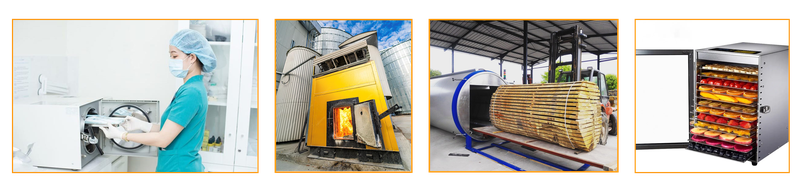
\includegraphics[width=12cm]{Images/ungdunghoahoi}
\end{center}
%\subsection*{III. Thí nghiệm}
%\setcounter{paragraph}{0}
%\subsubsection{Xác định nhiệt nóng chảy riêng của nước đá}
%\begin{itemize}
%	\item\textbf{Phương án 1} 
%\begin{itemize}
%	\item Cho một lượng nước có khối lượng $m_n$  và nhiệt dung riêng $c_n$  vào trong bình nhiệt lượng kế và que khuấy có khối lượng  $m_b$ và nhiệt dung riêng $c_b$. Ban đầu bình và nước ở nhiệt độ  $T_0$.
%	\item Thả vào bình một khối nước đá ở $0^\circ C$ có khối lượng $m_{nd}$, nhiệt nóng chảy riêng  $\lambda$. 
%	\item Khối nước đá nhận nhiệt lượng từ bình nhiệt lượng kế chứa nước để chuyển từ thể rắn sang thể lỏng ở  $0^\circ C\ (273K)$ sau đó tăng lên đến nhiệt độ T.
%	\item Bỏ qua nhiệt lượng toả ra của bình nhiệt lượng kế và que khuấy 
%	\begin{align*}
%		m_nc_n.\left(T_0-T\right)\approx \lambda.m_{nd}+m_{nd}c_n.\left(T-273\right)\Leftrightarrow \lambda=\dfrac{m_nc_n.\left(T-T_0\right)-m_{nd}.c_n.\left(T-273\right)}{m_{nd}}
%	\end{align*}
%	\item[a)] \textbf{Dụng cụ}
%	\begin{itemize}
%		\item 1 bình nhiệt lượng kế (có que khuấy).
%		\item Cốc nước đá.
%		\item 1 nhiệt kế có độ chia nhỏ nhất $1^\circ C$. 
%		\item 1 chiếc cân điện tử có độ chia nhỏ nhất 0,01 g.
%	\end{itemize}
%	\item[b)] \textbf{Tiến hành thí nghiệm} 
%\begin{itemize}
%	\item Bước 1: Điều chỉnh đơn vị đo của cân là g. Đặt bình nhiệt lượng kế (đã gắn nhiệt kế và que khuấy) lên đĩa cân, hiệu chỉnh cân về số 0,00.
%	\item Bước 2: 
%	\begin{itemize}
%		\item Nhấc bình nhiệt lượng kế khỏi đĩa cân, rót nước ở nhiệt độ phòng vào bình nhiệt lượng 	kế (khoảng $\dfrac{2}{3}$ bình).
%		\item Đặt bình nhiệt lượng kế lên đĩa cân, ghi giá trị khối lượng $m_n$  và nhiệt độ ban đầu  $T_0$	của nước.
%		\item Lặp lại phép đo khối lượng  $m_n$ thêm hai lần.
%	\end{itemize}
%\item Bước 3: Đặt bình nhiệt lượng kế chứa nước lên đĩa cân, hiệu chỉnh cân về số 0,00.
%\item Bước 4
%\begin{itemize}
%	\item Nhấc bình nhiệt lượng kế ra khỏi đĩa cân, cho khối nước đá vào bình nhiệt lượng kế.
%	\item Đậy kín nặp bình nhiệt lượng kế, dùng que khuấy đều đến khi nước đá tan hết. Ngay khi nước đá tan hết, ghi giá trị T của nước.
%\end{itemize}
%\item Bước 5: Đặt bình nhiệt lượng kế lên đĩa cân. Ghi giá trị $m_{nd}$ của khối nước đá. Lặp lại phép đo này thêm 2 lần
%\begin{center}
%	\begin{tabular}{|c|c|c|c|c|}
%		\hline 
%		Lần đo & $m_n\ (g)$ & $m_{nd}\ (g)$ &$T_0\ (K)$  &T (K)  \\ 
%		\hline 
%		1&  &  &  &  \\ 
%		\hline 
%		2&  &  &  &  \\ 
%		\hline 
%		3&  &  &  &  \\ 		\hline 
%		Giá trị trung bình&  &  &  &  \\ 
%				\hline 
%\end{tabular} 
%\end{center}
%\item Bước 6: Tính giá trị nhiệt nóng chảy riêng trung bình của nước đá.
%\begin{align*}
%	\overline{\lambda}=\dfrac{\overline{m_n}.c_n.\left(T_0-T\right)-\overline{m}_{nd}.c_{nd}.\left(T-273\right)}{\overline{m}_{nd}}
%\end{align*}
%\end{itemize}
%\end{itemize}
%\item \textbf{Phương án 2}
%\begin{itemize}
%	\item[a)] \textbf{Dụng cụ thí nghiệm}
%	\begin{itemize}
%		\item Sử dụng các dụng cụ như hình và chuẩn bị thêm các viên nước đá nhỏ.
%		\begin{center}
%			includegraphics[width=8cm]{Images/tn2}
%		\end{center}
%	\end{itemize}
%	\item[b)] \textbf{Tiến hành thí nghiệm}
%	  \begin{itemize}
%	  	\item Cho viên nước đá có khối lượng m (kg) và một ít nước lạnh vào bình nhiệt lượng kế, sao cho toàn bộ điện trở chìm trong hỗn hợp nước và nước đá.
%	  	\item Cắm đầu đo của nhiệt lượng kế vào bình nhiệt lượng kế.
%	  	\item Khuấy liên tục nước đá, cứ sau khoảng thời gian 2 phút đọc số đo trên oát kế và nhiệt độ trên nhiệt kế.
%	  	\item Vẽ đồ thị nhiệt độ t theo thời gian  $\tau$.
%	  			\begin{center}
%	  		\begin{tikzpicture}[scale=2,thick,>=stealth']
%	  			\tkzDefPoints{0/0/o, 5.5/0/x, 0/4.75/y, 3/0/m, 3.6/0.9/a, 4.225/2.1/b, 4.78/3.6/c}
%	  			\draw  [help  lines, xstep=0.5cm,ystep=0.5cm]  (0,0)  grid  (5.5,4.75);
%	  			\tkzDrawSegments[->](o,x o,y)
%	  			\tkzLabelPoint[left](o){$O$}
%	  			\tkzLabelPoint[above](x){$\tau\ (s)$}
%	  			\tkzLabelPoint[above](y){$t\ (^\circ C)$}
%	  			\draw[very thick,red] (3,0) -- (5.5,4.75);
%	  			
%	  			\foreach  \x  in  {1,2,...,9}
%	  			{\pgfmathtruncatemacro{\label}{100*\x};
%	  				\node[below, scale=0.9]
%	  				(\label) at (.5*\x,0) {\label};}
%	  			
%	  			\foreach \y[evaluate=\y as \text using .2*\y] in {1,...,8}{
%	  				\node at (0,.5*\y)[left=0pt,rotate = 0, scale=0.9] 
%	  				{\pgfmathprintnumber[fixed,fixed zerofill,precision=1]{\text}};
%	  			}
%	  			
%	  			\foreach  \x  in  {1,2,...,5}
%	  			{\pgfmathtruncatemacro{\label}{.6*\x};
%	  				\draw[fill=blue,blue](.6*\x,0)circle(0.6pt);}
%	  			\tkzLabelPoint[above left](m){$M$}
%	  			\tkzDrawPoints[size=3,fill=blue](a,b,c)
%	  		\end{tikzpicture}
%	  	\end{center}
%	  	\item Chọn điểm M là giao điểm của hai đường thẳng, đọc giá trị  $\tau_M$.
%	  	\item Tính công suất trung bình $\mathcal{P}$.
%	  	\item Tính nhiệt lượng nóng chảy riêng của nước đá theo công thức 
%	  	\begin{align*}
%	  		\lambda_{H_2O}=\dfrac{\mathcal{P}.\tau_M}{m}\quad \begin{cases}
%	  			m\ (kg):\  \text{khối lượng nước đá}\\
%	  			\mathcal{P}.\tau_M\ (J):\ \text{nhiệt lượng do dòng điện qua điện trở toả ra trong thời gian }\tau_M
%	  		\end{cases}
%	  	\end{align*}
%	  \end{itemize}
%\end{itemize}
%\item \textbf{Phương án 3}
%\begin{itemize}
%	\item Dòng diện làm nóng dây điện trở trong bình nhiệt lượng kế và làm nước đá nóng chảy. 
%	\item Khối lượng nước đá nóng chảy được hứng vào cốc và được xác định bằng cân.
%	\item Công suất điện tiêu thụ được xác định bằng oát kế. 
%	\item Tính nhiệt dung riêng bằng công thức sau: 
%	\begin{align*}
%\lambda=\dfrac{\mathcal{P}t}{M-2m}
%\begin{cases}
%	M\ (kg):\ \text{khối lượng của nước trong cốc sau khi bật nguồn trong thời gian t}
%	\\
%	m\ (kg):\ \text{khối lượng nước chảy vào cốc trong thời gian t (chưa bật nguồn)}\\
%	t\ (s:\ \text{thời gian đun}.)\\
%	\mathcal{P}:\ (W)\ \text{công suất}.
%\end{cases}
%	\end{align*}
%\end{itemize}
%\item[a)] \textbf{Dụng cụ}
%\begin{itemize}
%	\item Biến áp nguồn; Oát kế; Nhiệt lượng kế kèm dây điện trở; Cốc hứng nước và cân; Đồng hồ 
%\end{itemize}
%	  			\begin{center}
%	includegraphics[width=8cm]{Images/tn49}
%\end{center}
%\item[b)] \textbf{Tiến hành thí nghiệm}
%\begin{itemize}
%	\item Bước 1: Xác định khối lượng nước đá đã tan chảy m sau thời gian t (khi chưa bật nguồn)
%\begin{itemize}
%		\item Cho nước đá vào nhiệt lượng kế và hứng nước chảy ra bằng một chiếc cốc.
%		\item Sau khi nước chảy vào cốc khoảng một phút, cho nước chảy vào cốc trong thời gian t 	phút, xác định khối lượng m của nước trong cốc này.
%\end{itemize}
%\item Bước 2: Xác định khối lượng M của nước trong cốc (khi bật nguồn)
%\begin{itemize}
%	\item Bật biến áp nguồn.
%	\item Đọc số chỉ .$\mathcal{P}$  của oát kế.
%	\item Cho nước chảy thêm vào cốc trong thời gian t (phút).
%	\item Xác định khối lượng M của nước trong cốc lúc này.
%\end{itemize}
%\item Bước 3: Xác định nhiệt nóng chảy riêng của nước bằng công thức: 
%\begin{align*}
%	\lambda=\dfrac{\mathcal{P}t}{M-2m}
%\end{align*}
%\end{itemize}
%\end{itemize}
%\begin{note}
%	\begin{itemize}
%		\item Để xác định khối lượng nước đá đã tan chảy m sau thời gian t ở bước 1. Ta làm như sau
%		\begin{itemize}
%			\item Sau khi cho nước chảy vào cốc khoảng một phút, ta hiệu chỉnh cân về số 0. Bắt đầu bấm 	đồ hồ trong thời gian t phút. 
%			\item Đọc số chỉ của cân ta thu được khối lượng m của nước đá đã tan chảy trong t phút 
%		\end{itemize}
%		\item Khối lượng nước đá nóng chảy do nhận nhiệt lượng từ dây điện trở được xác định là (M-2m) vì
%\begin{itemize}
%	\item Ở bước 1, ta đã xác định được khối lượng m của nước đá đã tan chảy trong t phút
%	\item Sau đó ở bước 2, bật công tắc nguồn và cho nước đá chảy vào cốc trong thời gian đúng t 	phút. Trong quá trình này, ngoài nhiệt lượng nước đá nhận từ dây điện trở thì nó còn 	nhận nhiệt lượng từ môi trường như và tan chảy một khối lượng m (do đo đúng thời 	gian t như bước 1).
%	\item Vì vậy, khối lượng nước đá đã tan chảy do nhận nhiệt từ dây điện trở là  $(M-2m)$
%\end{itemize}
%	\end{itemize}
%\end{note}
%\subsubsection{Xác định nhiệt hoá hơi riêng}
%\begin{itemize}
%	\item \textbf{Phương án 1}
%	\begin{itemize}
%		\item Cho một lượng nước vào ấm đun có công suất $\mathcal{P}$. Cấp dòng điện xoay chiều cho ấm đun. Khi nước sôi, mở nắp ấm đun để nước bay hơi ra ngoài làm khối lượng nước giảm dần.
%		\item Gọi $\Delta m$ là khối lượng nước bị bay hơi sau thời gian t, L là nhiệt hoá hơi riêng của nước ở nhiệt độ sôi. Ta có:
%		\begin{align*}
%			L.\Delta m=\mathcal{P}\tau\quad 
%			\begin{cases}
%				m\ (kg):\ \textbf{khối lượng của vật}\\
%				L\ (J/kg):\ \textbf{nhiệt hoá hơi riêng}\\
%				\mathcal{P}\ (J):\ \textbf{công suất của ấm đun}\\
%				\tau\ (s):\ \textbf{thời gian đun}
%			\end{cases}
%		\end{align*}
%	\item[a)] Dụng cụ đo
%	\begin{itemize}
%		\item 1 chiếc cân điện tử có độ chia nhỏ nhất 0,01 g.
%		\item 1 ấm đun nước siêu tốc loại 1,8 lít.
%		\item 1 đồng hồ đo thời gian có độ chia nhỏ nhất 0,01 s.
%		\item 1 chai nước ở nhiệt độ phòng.
%	\end{itemize}
%		\item[b)] \textbf{Tiến hành thí nghiệm}
%		\begin{itemize}
%					\item Bước 1: Xác định khối lượng nước trong ấm
%					\begin{itemize}
%						\item Điều chỉnh đơn vị đo của cân là g. Đặt ấm đun lên đĩa cân, hiểu chỉnh cân về số 0,00
%						\item Rót nước từ từ vào ấm đun đến giá trị khoảng 320,00 g.
%					\end{itemize}
%				\item Bước 2: Đun nước sôi
%				\begin{itemize}
%					\item Đặt ấm đun lên đĩa cân, bật công tắc để bắt đầu đun nước. Khi nước vừa sôi, mở nắp 	ấm đun để nước bay hơi. 
%					\item Khi thấy cân địa tử chỉ 300,00 g thì bắt đầu bấm đồng hồ đo thời gian. 
%				\end{itemize}
%			\item Bước 3: Đọc khối lượng nước và thời gian
%			\begin{itemize}
%				\item Khi thấy số chỉ trên cân giảm còn 250,00 g (khối lượng nước còn lại) thì ghi thời gian $\tau\ (s)$	  và khối lượng m theo bảng dưới
%				\item Lặp lại phép đo  $\tau\ (s)$ và  m khi số chỉ trên cân điện tử lần lượt giảm còn 200,00 g và 150,00 g
%			\end{itemize}
%		\end{itemize}
%			\end{itemize}
%		\begin{center}
%			\begin{tabular}{|c|c|c|c|c|}
%				\hline 
%				Lần đo & $m_n\ (g)$ & $\Delta m=m-m_0\ (g)$ &$\tau\ (s)$  &L (J/g)  \\ 
%				\hline 
%				1&  &  &  &  \\ 
%				\hline 
%				2&  &  &  &  \\ 
%				\hline 
%				3&  &  &  &  \\ 		\hline 
%				Giá trị trung bình&  &  &  &  \\ 
%				\hline 
%			\end{tabular} 
%		\end{center}
%\item \textbf{Phương án 2}
%	\begin{itemize}
%		\item[a)] \textbf{Dụng cụ thí nghiệm}
%		\begin{itemize}
%			\item Sử dụng các dụng cụ như hình và chuẩn bị thêm một lượng nước nóng
%		\end{itemize} 
%	\item[b)] \textbf{Tiến hành thí nghiệm}
%	\begin{itemize}
%		\item Đặt bình nhiệt lượng kế lên cân. Đổ nước nóng vào nhiệt lượng kế. Xác định khối lượng nước trong bình
%		\item Mở nắp bình nhiệt lượng kế, nối oát kế với điện trở và nguồn điện.
%		\item Đặt dây điện trở và nhiệt lượng kế sao cho toàn bộ dây chìm trong nước.
%		\item Bật nguồn điện.
%		\item Đun sôi nước trong bình nhiệt lượng kế. Sau mỗi khoảng thời gian 2 phút, đọc số đo công suất trên oát kế, khối lượng nước trong bình nhiệt lượng kế trên cân. Ghi các kết quả vào bảng
%		\item Tắt nguồn điện.
%		\begin{center}
%			\begin{tabular}{|c|c|c|c|c|c|c|c|c|}
%				\hline 
%				Thời gian $\tau\ (s)$ & 0 & 120  &240  &360&480&600&720&840\\ \hline  
%			 Công suất $\mathcal{P}\ (W)$&  &   &&&&&&  		\\ 		\hline 
%			 Khối lượng $m\ (kg)$&  &   &&&&&&  		\\ 		\hline 
%		\end{tabular} 
%		\end{center}
%		\item Vẽ đồ thị khối lượng m theo thời gian $\tau$.
%			  			\begin{center}
%			includegraphics[width=8cm]{Images/dt11}
%		\end{center}
%		\item Chọn hai điểm P và Q tuỳ ý trên đồ thị, xác định khối lượng  $m_P,\ m_Q$ và thời gian $\tau_P,\ \tau_Q$   
%		\item Tính công suất trung bình của dòng điện qua điện trở của nhiệt lượng kế
%		\item  Tính nhiệt hoá hơi riêng của nước theo công thức 
%		\begin{align*}
%			L=\dfrac{Q}{m}=\dfrac{\overline{\mathcal{P}}.\left(\tau_Q-\tau_P\right)}{m_P-m_Q}\quad 
%			\begin{cases}
%				\left(m_P-m_Q\right)\ (kg):\ \text{khối lượng của nước đã hoá hơi}\\
%				\overline{\mathcal{P}}.\left(\tau_Q-\tau_P\right):\ \text{nhiệt lượng do dòng điện qua}\\ 
%				\text{điện trở toả ra trong khoảng thời gian $(\tau_Q-\tau_P)$}
%			\end{cases}
%		\end{align*}
%	\end{itemize} 
%	\end{itemize}
%\end{itemize}
\subsection{ĐỒ THỊ MÔ TẢ QUÁ TRÌNH CHUYỂN THỂ CỦA NƯỚC Ở ÁP SUẤT 1 ATM}
\begin{center}
	\begin{tikzpicture}[scale=1,thick,>=stealth']
		\tkzDefPoints{0/0/o, 15/0/x, 0/9/y, 0/1.5/ay, 0/3/by, 0/6.5/cy, 0/7.5/ey, 2/3/a, 2/0/a', 4.5/3/b, 4.5/0/b', 7.5/6.5/c, 7.5/0/c', 11/6.5/d, 11/0/d', 13.75/9/e, 13.75/0/e'}
		\draw[fill=blue!50,blue!50] (ay) -- (a) -- (a') -- (o);
		\draw[purple!5, fill=purple!5] (a) -- (b) -- (b') -- (a') -- (a);
		\draw[fill=cyan!30,cyan!30] (b) -- (c) -- (c') -- (b');
		\draw[fill=blue!20,blue!20] (c) -- (d) -- (d') -- (c') -- (c);
		\draw[fill=green!30, green!30] (d) -- (e) -- (e') -- (d') -- (d);
		\tkzDrawSegments[thick,->](o,x o,y)
		\draw (ay) -- (a) -- (b) -- (c) -- (d) -- (e);
		\draw[dashed,thin] (a) -- (a')(b) -- (b')(c) -- (c')(d) -- (d')(e) -- (e')(a) -- (by)(c) -- (cy);
		\tkzDrawPoints[size=5,fill=white](o,cy, a,b,c,d,e,by)
		\tkzDrawPoints[size=4,fill=white](a',b',c',d',e')
		\tkzLabelPoint[below](x){Q (J)}
		\tkzLabelPoint[above](y){t ($^\circ C$)}
		\tkzLabelPoint[left](by){$0$}
		\tkzLabelPoint[left](cy){$100$}
		\node at (1,0.25) {$Q=mc.\Delta t$};
		\node at (3.25,0.25) {$Q=\lambda .m$};
		\node at (6,0.25) {$Q=mc.\Delta t$};
		\node at (9.25,0.25) {$Q=L.m$};
		\node at (12.5,0.25) {$Q=mc.\Delta t$};
		\node[inner sep=0pt,yshift=0pt] at (1,1.25){
\includegraphics[width=1.5cm]{Images/Ran}};
		\node[inner sep=0pt,yshift=0pt] at (3.25,1.75){
\includegraphics[width=2.5cm]{Images/RanLong}};
		\node[inner sep=0pt,yshift=0pt] at (6,2.5){
\includegraphics[width=3cm]{Images/Long}};
		\node[inner sep=0pt,yshift=0pt] at (9.3,3.25){
\includegraphics[width=2.5cm]{Images/LongKhi}};
		\node[inner sep=0pt,yshift=0pt] at (12.25,4.75){
\includegraphics[width=4.5cm]{Images/Khi}};
		\tkzLabelSegment[above,sloped](ay,a){Rắn}
		\tkzLabelSegment[above,sloped](a,b){Nóng chảy}
		\tkzLabelSegment[above,sloped](b,c){Lỏng}
		\tkzLabelSegment[above,sloped](c,d){Hóa hơi}
		\tkzLabelSegment[above,sloped](d,e){Hơi}
	\end{tikzpicture}
\end{center}